\documentclass[a4paper]{article}

%% Language and font encodings
\usepackage[english]{babel}
\usepackage[utf8x]{inputenc}
\usepackage[T1]{fontenc}
\usepackage{caption}

%% Sets page size and margins
\usepackage[a4paper,top=3cm,bottom=2cm,left=3cm,right=3cm,marginparwidth=1.75cm]{geometry}

%% Useful packages
\usepackage{amsmath}
\usepackage{amsfonts}

\usepackage{graphicx}
\usepackage{tikz}
\usetikzlibrary{arrows.meta}

\usepackage[colorinlistoftodos]{todonotes}
\usepackage[colorlinks=true, allcolors=blue]{hyperref}

\usepackage{color}
\usepackage{url}

%% display solutions or not
\newif\ifsol
\soltrue % comment out to hide solutions

%% todo tracker -- overleaf v2 has better one it uses but will default to this if compiled on something that doesn't have built-in todo
\newcommand{\todo}[1]{\textbf{\textcolor{red}{#1}}}

\title{Section 4: CSPs and Local Search}
\author{CS 182 - Artificial Intelligence}
\date{}

\begin{document}
\maketitle

\noindent \textbf{CSPs} are formalized as a triple $\langle X,D,C \rangle$. 
\begin{enumerate}
\item $X = \{X_1, \ldots, X_n\}$: A set of variables in the problem
\item $D = \{D_1, \ldots, D_n\}$: The domains for these variables
\item $C = \{C_1, \ldots, C_m\}$: Constraints
\end{enumerate}
Constraints encode the limits on the values/domains for each variable contingent on the values/domains of other variables.
\\ \\
\noindent One way to solve a CSP is through \textbf{backtracking search} which is simply DFS with two changes:
\begin{enumerate}
\item Fix the variable ordering ($X_1 = D_1 \rightarrow X_2 = D_2 \equiv X_2 = D_2 \rightarrow X_1 = D_1$).
\item Check constraints as you go and backtrack if you violate any.
\end{enumerate}
One way to optimize this process is to use the most constrained variable (the variable with the minimum remaining values) and assign the least constraining variable. Another optimization is to use \textbf{forward checking} to do a one step check for inconsistent solutions at each assignment. Finally one can use \textbf{arc consistency} to check the entire chain of implications of one assignment.
\\ \\
\noindent \textbf{Optimization} is the process of computing an optimal solution (e.g., min cost, max reward) to some mathematical problem. Optimization is often used to solve complex problems as it casts a real world problem into a simple math problem which can be solved via off-the-shelf solvers. Unfortunately, many optimization problems are NP-complete. Therefore, globally optimal solutions cannot often be found and instead locally optimal solutions are searched for from some (ideally) informed initial condition. \textbf{Local Search Algorithms} include:
\begin{enumerate}
    \item \textbf{Hill Climbing} is the simplest approach. Given a state $s$, generate all successors $s'$ and move to the best one. If there is no better successor, return the current state. A variant of this allows for \textbf{random restarts} to try to escape local minimums.
    \item \textbf{Simulated Annealing} picks a random successor state at each step. If the random successor is better, the state moves. If it is worse, it is accepted with probability $\exp(\Delta E / T)$. The algorithm starts with large $T$ (exploration) and decreases it over time. 
    \item In \textbf{Beam Search}, we choose $k$ random initial states. All successors for all $k$ states are expanded. Among all of the generated states, the best $k$ states are chosen. 
    \item \textbf{Genetic Algorithms} start with a set of possible solutions. Inspired by natural selection, at each iteration, a biased sample (based on a measure of ``fitness'') is taken from the current solution set. A new solution set is then constructed by ``crossing over'' (aka combining parts of) pairs of sampled solutions. ``Mutation'' (aka random changes to solutions) are also added during iterations. These algorithms can avoid local minima but may take many iterations to converge to a good solution.
    \item \textbf{Gradient Descent} relies on an assumption that we are minimizing a locally convex (or maximizing a locally concave) function. It takes the gradient, the partial derivatives, of the function which points in the direction of maximum descent (ascent) and moves in that direction iteratively, $x_{t+1} = x_t - \alpha \nabla f(x)$, until it reaches a local minimum (maximum) where $\nabla f(x) = 0$. \textbf{Stochastic Gradient Descent} approximates the gradient through sampling and is otherwise the same. $x_{t+1} = x_t - \alpha \left(f(x+w) - f(x)\right)w$ for $w \sim \mathcal{N}(0,\,\Sigma)$. These are both used in continuous domains.
\end{enumerate}

\clearpage
\section*{Practice Problems}
\begin{enumerate}
\item Pacman is trapped!\footnote{From Berkeley Section material} He is surrounded by mysterious corridors, each of which leads to either a pit (P), a ghost (G), or an exit (E). In order to escape, he needs to figure out which corridors, if any, lead to an exit and freedom,
rather than the certain doom of a pit or a ghost.

The one sign of what lies behind the corridors is the wind: a pit produces a strong breeze (S) and an exit produces a weak breeze (W), while a ghost doesn’t produce any breeze at all. Unfortunately, Pacman cannot measure the strength of the breeze at a specific corridor. Instead, he can stand between two adjacent corridors and feel the max of the two breezes. For example, if he stands between a pit and an exit he will sense a strong (S) breeze, while if he stands between an exit and a ghost, he will sense a weak (W) breeze. The measurements for all intersections are shown in the figure below. Also, while the total number of exits might be zero, one, or more, Pacman knows that two neighboring squares will not both be exits.

\begin{figure}[h]
\centering
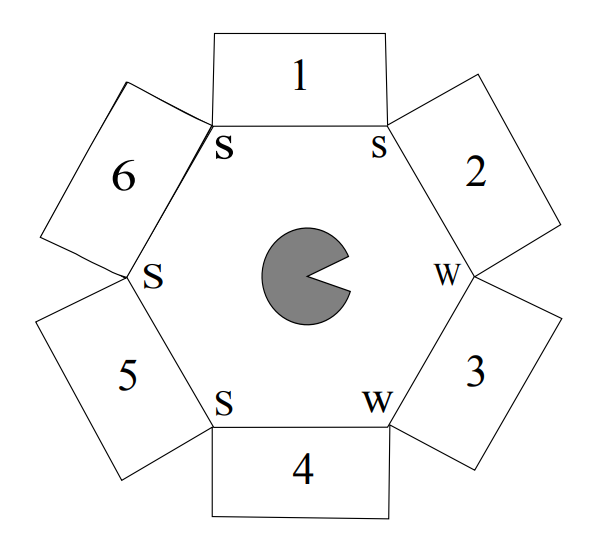
\includegraphics[width=0.33\textwidth]{figs/pacman-prob}
\end{figure}

Pacman models this using variables $X_i$ for each corridor $i$ and domains $P$, $G$, and $E$.

\begin{enumerate}
\item State the binary and/or unary constraints for this CSP (either implicitly or explicitly).
\ifsol
    \begin{figure}[h]
    \centering
    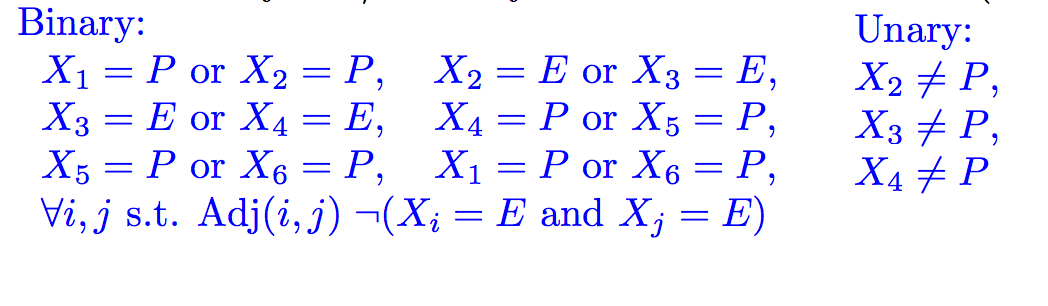
\includegraphics[width=0.5\textwidth]{figs/constraints-sol}
    \end{figure}
\else
    \vspace{8em}
\fi

\item Cross out / remove the values from the domains of the variables that will be deleted by forward checking from the initial constraints (part a). What about arc consistency?

\ifsol
    \begin{figure}[h]
    \centering
    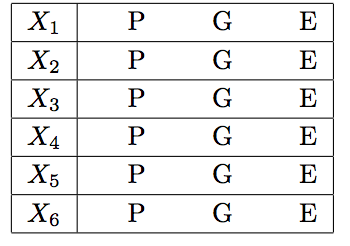
\includegraphics[width=0.31\textwidth]{figs/forward-options}
    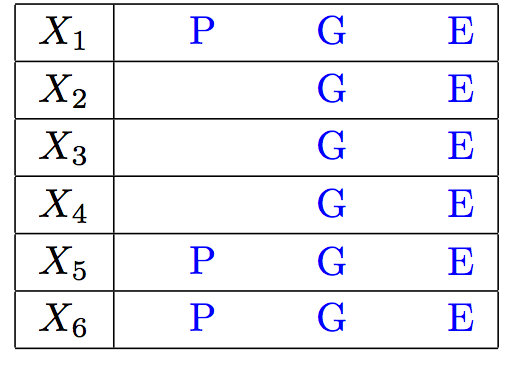
\includegraphics[width=0.3\textwidth]{figs/forward-sol2}
    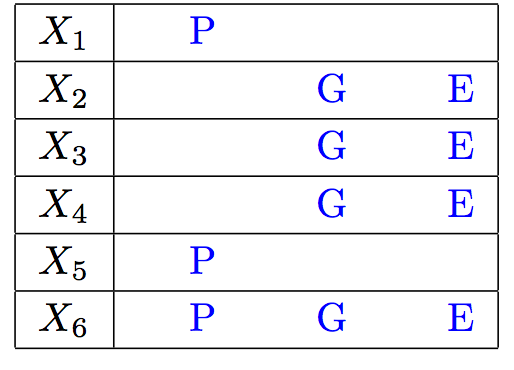
\includegraphics[width=0.3\textwidth]{figs/forward-sol}
    \vspace{-1em}
    \captionsetup{labelformat=empty}
    \caption{Initial Domain \quad \quad \quad \quad Forward Checking \quad \quad \quad \quad \quad Arc Consistency}
    \vspace{-1em}
    \end{figure}
\else
    \begin{figure}[h]
    \centering
    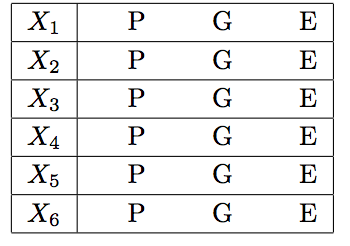
\includegraphics[width=0.33\textwidth]{figs/forward-options}
    \end{figure}
\fi

\item According to minimum remaining values (MRV), which variable or variables could the solver assign first?

\ifsol
    \textcolor{blue}{$X_1$ or $X_5$ (tie breaking)}
\else
    \vspace{3em}
\fi

\item Assume that Pacman knows that $X_6 = G$. List all the solutions of this CSP or write none if no solutions exist.

\ifsol
    \textcolor{blue}{(P,E,G,E,P,G)\linebreak(P,G,E,G,P,G)}
\else
    \vspace{3em}
\fi

\end{enumerate}

\item Consider the graph with 8 nodes $A_1$, $A_2$, $A_3$, $A_4$, $H$, $T$, $F_1$, $F_2$. $A_i$ is connected to $A_{i+1}$ for all $i \in [1, 2, 3]$, each $A_i$ is connected to $H$, $H$ is connected to $T$, and $T$ is connected to each $F_i$. Find a 3-coloring of this graph by hand using the following strategy: backtracking with conflict-directed backjumping, the variable order $A_1$, $H$, $A_4$, $F_1$, $A_2$, $F_2$, $A_3$, $T$, and the value order $R$, $G$, $B$.
\ifsol
    \textcolor{blue}{\begin{enumerate}
    \item $A_1 = R$.
    \item $H = R$ conflicts with $A_1$.
    \item $H = G$.
    \item $A_4 = R$.
    \item $F_1 = R$.
    \item $A_2$ = R; conflicts with $A_1$, $A_2 = G$ conflicts with $H$, so $A_2 = B$.
    \item $F_2 = R$.
    \item $A_3 = R$ conflicts with $A_4$, $A_3 = G$ conflicts with $H$, $A_3 = B$ conflicts with $A_2$, so backtrack. Conflict set is $\{A_2, H, A_4\}$, so we jump back to $A_2$.
    \item $A_2$ has no more values it can take outside of the current $B$, so backtrack again. Full conflict set is $\{A_1, H, A_4\}$ so jump back to $A_4$.
    \item $A_4 = G$ conflicts with $H$, so $A_4 = B$.
    \item $F_1 = R$.
    \item $A_2 = R$ conflicts with $A_1$, $A_2 = G$ conflicts with $H$, so $A_2 = B$.
    \item $F_2 = R$.
    \item $A_3 = R$.
    \item $T =R$ conflicts with $F_1$ and $F_2$, $T = G$ conflicts with $G$, so $T = B$. 
    \item Success!
    \end{enumerate}}
\else
    \vspace{25em}
\fi



\item Consider the problem of placing $k$ knights on an $n \times n$ chessboard such that no two knights are attacking each other, where $k$ is given and $k \leq n^2$.
\begin{enumerate}
\item Choose a CSP formulation. In your formulation, what are the variables? What is the domain for each variable?

\ifsol
    \textcolor{blue}{ There are two solutions. (a) Each position in the board is a variable. Each variable can take a binary value indicating whether the field is occupied. (b) Each knight is a variable, every variable's domain is the set of squares on the board.}
\else
    \vspace{5em}
\fi

\item What are the constraints?

\ifsol
    \textcolor{blue}{ (a) Every pair of squares separated by a knight’s move is constrained, such that both cannot be occupied. Furthermore, the entire set of squares is constrained, such that the total number of occupied squares should be $k$.\newline
    (b) Every pair of knights is constrained, such that no two knights can be on the same square or on squares separated by a knight’s move. Solution B lacks the global constraint, although Solution A has the smaller state space for large $k$. }
\else
    \vspace{7em}
\fi

\item Now consider the problem of putting as many knights as possible on the board without any attacks. Explain how to solve this with local search by defining appropriate actions and a sensible objective function. \textbf{Note}: Don't try to solve this problem, only lay out the strategy.

\ifsol
    \textcolor{blue}{Any solution must describe a \emph{complete-state} formulation because we are using a local search algorithm. For simulated annealing, the successor function must completely connect the space; for random-restart, the goal state must be reachable by hill climbing from some initial state. \newline
    Two approaches are:
    \begin{itemize}
    \item Ensure no conflicts at any time. Actions are to remove any knight, add a knight in any unattacked square, or move a knight to any unattacked square.
    \item Allow conflicts but try to get rid of them. Actions are to remove any knight, add a knight in any square, or move a knight to any square.
    \end{itemize}}
\else
    \vspace{15em}
\fi
\end{enumerate}

\item Given the function shown in the Figure below, what are the solution for hill climbing and simulated annealing with the starting points $x = 1$, $x = 4$ and $x = 5$? Additionally give the solution for a Beam Search with $k = 3$ and starting points $2$, $4$ and $6$.\footnote{from University of Hildesheim}

\begin{figure}[h]
\centering
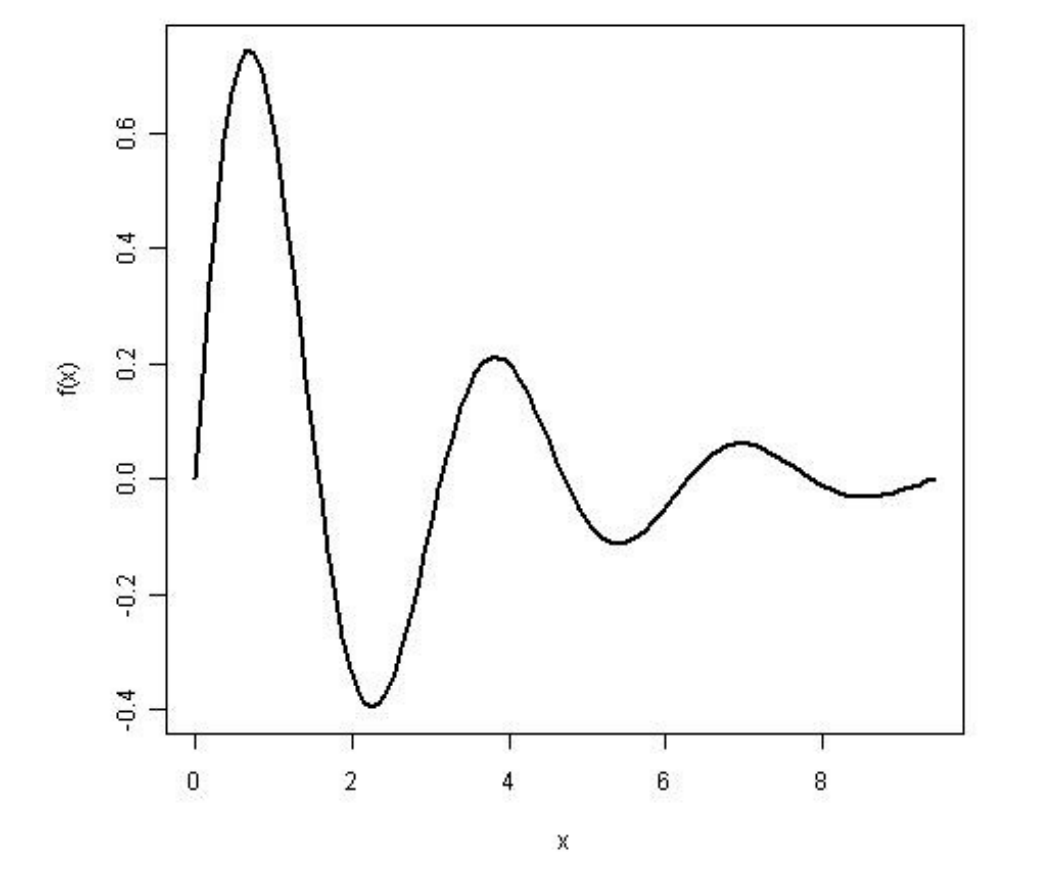
\includegraphics[width=0.5\textwidth]{figs/climbing}
\end{figure}

\ifsol
    \textcolor{blue}{
    \begin{itemize}
    \item $x = 1$: HC: 1, SA: ? (but hopefully 1 or we have a really bad temperature function)
    \item $x = 4$: HC: 4, SA: ? (depends on temperature)
    \item $x = 5$: HC = 4, SA: ? (depends on temperature)
    \item $x = {2,4,6}$: BS: 4 
    \end{itemize}}
\else
    \vspace{7em}
\fi

\item Give the name of the algorithm that results from each of the following special cases:
\begin{enumerate}
\item Local beam search with $k = 1$.

\ifsol
    \textcolor{blue}{Local beam search with $k = 1$ is hill-climbing search.}
\else
    \vspace{5em}
\fi

\item Local beam search with one initial state and no limit on the number of states retained.

\ifsol
    \textcolor{blue}{Local beam search with one initial state and no limit on the number of states retained, resembles BFS in that it adds one complete layer of nodes before adding the next layer. Starting from one state, the algorithm would be essentially identical to BFS except that each layer is generated all at once.}
\else
    \vspace{5em}
\fi

\item Simulated annealing with $T = \infty$ at all times.

\ifsol
    \textcolor{blue}{Simulated annealing with $T = \infty$ at all times is a random-walk search: it always accepts a new state.}
\else
    \vspace{5em}
\fi

\item Genetic algorithm with population size $N = 1$.

\ifsol
    \textcolor{blue}{If the population size is 1, then the two selected parents will be the same individual; crossover yields an exact copy of the individual; then there is a small chance of mutation. Thus, the algorithm executes a random walk in the space of individuals.}
\else
    \vspace{5em}
\fi
\end{enumerate}
\newpage

\item In (neural network) machine translation, you have a fully differentiable function $f$ with a set of continuous parameters $\theta \in \mathbb{R}^N$ that predicts an output sequence $\textbf{y}$ from an input sequence $\textbf{x}$. You have a corpus with sentences in English ($\textbf{X}$) and corresponding translations in Spanish ($\textbf{Y}$). Your goal is to find a set of parameters $\theta$ that maximizes $p(\textbf{y}|\textbf{x},\theta)$.
\begin{enumerate}
\item Formalize this problem as a local search problem. What is a state? What are possible successor states? 

\ifsol
    \textcolor{blue}{Every set of parameters is a possible state. Since we are operating in continuous space, any change in the parameters can be a possible successor.}
\else
    \vspace{3em}
\fi

\item Which algorithm from lecture could we use to find the best state? Is there a problem with this algorithm?

\ifsol
    \textcolor{blue}{An algorithm from lecture that can be used is (stochastic) gradient descent. Since $f$ is fully differentiable, we can calculate the gradient with respect to its input and use the gradient to compute updates to the parameters. There is a problem here though! The problem does not specify that the search space is convex and stochastic gradient descent can only yield a global maximum in convex space. In practice, it is still commonly used, since local maxima are ``good enough'' (more about this later in the course).}
\else
    \vspace{5em}
\fi

\end{enumerate}

Now that you successfully found a good $\theta$, you are given an unknown sentence $\textbf{x}$ and the task to translate it. You realize that while you can successfully assign a score to a pair of sentences $\textbf{x}$ and $\textbf{y}$, you still a way need to find the best $\textbf{y}$. 

\begin{enumerate}
\setcounter{enumii}{2}
\item Formalize the problem of finding the best sequence of output words $\textbf{y} = w_1, \ldots, w_l$ as a search problem. What is a state? What is a successor state? What is a goal state? Note that ``word'' in this context can also mean a special character.

\ifsol
    \textcolor{blue}{One possible way of formalizing this problem is to define a state as a sequence of input words $w_1, \ldots, w_n$, and a sequence of output words $W_1, \ldots, W_k$. The function $f$ is used to assign a score to this state. A successor state is a word $W_{k+1}$ that is appended to the output. Goal states are all sequences that end in a word that ends the sentence, such as ``.'', ``,'', ``?'', and ``!''.}
\else
    \vspace{5em}
\fi

\item How many states do you need to expand at each search step?

\ifsol
    \textcolor{blue}{We need to expand all possible words that our function knows about, also called vocabulary $\mathcal{V}$, at each step. The search space grows exponentially with length $l$ of the sequence  $|\mathcal{V}|^l$.}
\else
    \vspace{5em}
\fi

\end{enumerate}

A property of $f$ is that the score of each word in the output depends not only on the input $\textbf{x}$, but also on all previously generated words in $\textbf{y}$.

\begin{enumerate}
\setcounter{enumii}{4}
\item What does property this imply for your search algorithm choice?

\ifsol
    \textcolor{blue}{If generating a certain word would solely depend on an input, we could use a greedy hill-climbing algorithm to find the best output. However, since this is not the case, our search space likely contains many local maxima and we need to use different methods.}
\else
    \vspace{5em}
\fi

\item Suggest a search algorithm to tackle this problem, and discuss possible drawbacks of using this approach over others. 

\ifsol
    \textcolor{blue}{A possible approach to tackle this problem is to use Beam Search. Here, we keep the best $k$ hypotheses after each expansion. This makes sure that we don't choose locally-good, but globally-bad words. However, a possible drawback of this approach is that it generates boring sentences that all look very much alike with only few words differing. People address this problem typically by enforcing beams to be diverse from another (this is beyond the course material).}
\else
    \vspace{5em}
\fi
\end{enumerate}

\end{enumerate}
\end{document}